% Options for packages loaded elsewhere
\PassOptionsToPackage{unicode}{hyperref}
\PassOptionsToPackage{hyphens}{url}
%
\documentclass[
]{book}
\usepackage{amsmath,amssymb}
\usepackage{lmodern}
\usepackage{iftex}
\ifPDFTeX
  \usepackage[T1]{fontenc}
  \usepackage[utf8]{inputenc}
  \usepackage{textcomp} % provide euro and other symbols
\else % if luatex or xetex
  \usepackage{unicode-math}
  \defaultfontfeatures{Scale=MatchLowercase}
  \defaultfontfeatures[\rmfamily]{Ligatures=TeX,Scale=1}
\fi
% Use upquote if available, for straight quotes in verbatim environments
\IfFileExists{upquote.sty}{\usepackage{upquote}}{}
\IfFileExists{microtype.sty}{% use microtype if available
  \usepackage[]{microtype}
  \UseMicrotypeSet[protrusion]{basicmath} % disable protrusion for tt fonts
}{}
\makeatletter
\@ifundefined{KOMAClassName}{% if non-KOMA class
  \IfFileExists{parskip.sty}{%
    \usepackage{parskip}
  }{% else
    \setlength{\parindent}{0pt}
    \setlength{\parskip}{6pt plus 2pt minus 1pt}}
}{% if KOMA class
  \KOMAoptions{parskip=half}}
\makeatother
\usepackage{xcolor}
\usepackage{color}
\usepackage{fancyvrb}
\newcommand{\VerbBar}{|}
\newcommand{\VERB}{\Verb[commandchars=\\\{\}]}
\DefineVerbatimEnvironment{Highlighting}{Verbatim}{commandchars=\\\{\}}
% Add ',fontsize=\small' for more characters per line
\usepackage{framed}
\definecolor{shadecolor}{RGB}{248,248,248}
\newenvironment{Shaded}{\begin{snugshade}}{\end{snugshade}}
\newcommand{\AlertTok}[1]{\textcolor[rgb]{0.94,0.16,0.16}{#1}}
\newcommand{\AnnotationTok}[1]{\textcolor[rgb]{0.56,0.35,0.01}{\textbf{\textit{#1}}}}
\newcommand{\AttributeTok}[1]{\textcolor[rgb]{0.77,0.63,0.00}{#1}}
\newcommand{\BaseNTok}[1]{\textcolor[rgb]{0.00,0.00,0.81}{#1}}
\newcommand{\BuiltInTok}[1]{#1}
\newcommand{\CharTok}[1]{\textcolor[rgb]{0.31,0.60,0.02}{#1}}
\newcommand{\CommentTok}[1]{\textcolor[rgb]{0.56,0.35,0.01}{\textit{#1}}}
\newcommand{\CommentVarTok}[1]{\textcolor[rgb]{0.56,0.35,0.01}{\textbf{\textit{#1}}}}
\newcommand{\ConstantTok}[1]{\textcolor[rgb]{0.00,0.00,0.00}{#1}}
\newcommand{\ControlFlowTok}[1]{\textcolor[rgb]{0.13,0.29,0.53}{\textbf{#1}}}
\newcommand{\DataTypeTok}[1]{\textcolor[rgb]{0.13,0.29,0.53}{#1}}
\newcommand{\DecValTok}[1]{\textcolor[rgb]{0.00,0.00,0.81}{#1}}
\newcommand{\DocumentationTok}[1]{\textcolor[rgb]{0.56,0.35,0.01}{\textbf{\textit{#1}}}}
\newcommand{\ErrorTok}[1]{\textcolor[rgb]{0.64,0.00,0.00}{\textbf{#1}}}
\newcommand{\ExtensionTok}[1]{#1}
\newcommand{\FloatTok}[1]{\textcolor[rgb]{0.00,0.00,0.81}{#1}}
\newcommand{\FunctionTok}[1]{\textcolor[rgb]{0.00,0.00,0.00}{#1}}
\newcommand{\ImportTok}[1]{#1}
\newcommand{\InformationTok}[1]{\textcolor[rgb]{0.56,0.35,0.01}{\textbf{\textit{#1}}}}
\newcommand{\KeywordTok}[1]{\textcolor[rgb]{0.13,0.29,0.53}{\textbf{#1}}}
\newcommand{\NormalTok}[1]{#1}
\newcommand{\OperatorTok}[1]{\textcolor[rgb]{0.81,0.36,0.00}{\textbf{#1}}}
\newcommand{\OtherTok}[1]{\textcolor[rgb]{0.56,0.35,0.01}{#1}}
\newcommand{\PreprocessorTok}[1]{\textcolor[rgb]{0.56,0.35,0.01}{\textit{#1}}}
\newcommand{\RegionMarkerTok}[1]{#1}
\newcommand{\SpecialCharTok}[1]{\textcolor[rgb]{0.00,0.00,0.00}{#1}}
\newcommand{\SpecialStringTok}[1]{\textcolor[rgb]{0.31,0.60,0.02}{#1}}
\newcommand{\StringTok}[1]{\textcolor[rgb]{0.31,0.60,0.02}{#1}}
\newcommand{\VariableTok}[1]{\textcolor[rgb]{0.00,0.00,0.00}{#1}}
\newcommand{\VerbatimStringTok}[1]{\textcolor[rgb]{0.31,0.60,0.02}{#1}}
\newcommand{\WarningTok}[1]{\textcolor[rgb]{0.56,0.35,0.01}{\textbf{\textit{#1}}}}
\usepackage{longtable,booktabs,array}
\usepackage{calc} % for calculating minipage widths
% Correct order of tables after \paragraph or \subparagraph
\usepackage{etoolbox}
\makeatletter
\patchcmd\longtable{\par}{\if@noskipsec\mbox{}\fi\par}{}{}
\makeatother
% Allow footnotes in longtable head/foot
\IfFileExists{footnotehyper.sty}{\usepackage{footnotehyper}}{\usepackage{footnote}}
\makesavenoteenv{longtable}
\usepackage{graphicx}
\makeatletter
\def\maxwidth{\ifdim\Gin@nat@width>\linewidth\linewidth\else\Gin@nat@width\fi}
\def\maxheight{\ifdim\Gin@nat@height>\textheight\textheight\else\Gin@nat@height\fi}
\makeatother
% Scale images if necessary, so that they will not overflow the page
% margins by default, and it is still possible to overwrite the defaults
% using explicit options in \includegraphics[width, height, ...]{}
\setkeys{Gin}{width=\maxwidth,height=\maxheight,keepaspectratio}
% Set default figure placement to htbp
\makeatletter
\def\fps@figure{htbp}
\makeatother
\setlength{\emergencystretch}{3em} % prevent overfull lines
\providecommand{\tightlist}{%
  \setlength{\itemsep}{0pt}\setlength{\parskip}{0pt}}
\setcounter{secnumdepth}{5}
\usepackage{booktabs}
\ifLuaTeX
  \usepackage{selnolig}  % disable illegal ligatures
\fi
\usepackage[]{natbib}
\bibliographystyle{plainnat}
\IfFileExists{bookmark.sty}{\usepackage{bookmark}}{\usepackage{hyperref}}
\IfFileExists{xurl.sty}{\usepackage{xurl}}{} % add URL line breaks if available
\urlstyle{same} % disable monospaced font for URLs
\hypersetup{
  pdftitle={Relatório POAT},
  pdfauthor={Hidelbrando Ferreira Rodrigues},
  hidelinks,
  pdfcreator={LaTeX via pandoc}}

\title{Relatório POAT}
\author{Hidelbrando Ferreira Rodrigues}
\date{2022-09-15}

\usepackage{amsthm}
\newtheorem{theorem}{Theorem}[chapter]
\newtheorem{lemma}{Lemma}[chapter]
\newtheorem{corollary}{Corollary}[chapter]
\newtheorem{proposition}{Proposition}[chapter]
\newtheorem{conjecture}{Conjecture}[chapter]
\theoremstyle{definition}
\newtheorem{definition}{Definition}[chapter]
\theoremstyle{definition}
\newtheorem{example}{Example}[chapter]
\theoremstyle{definition}
\newtheorem{exercise}{Exercise}[chapter]
\theoremstyle{definition}
\newtheorem{hypothesis}{Hypothesis}[chapter]
\theoremstyle{remark}
\newtheorem*{remark}{Remark}
\newtheorem*{solution}{Solution}
\begin{document}
\maketitle

{
\setcounter{tocdepth}{1}
\tableofcontents
}
\hypertarget{introduuxe7uxe3o}{%
\chapter{Introdução}\label{introduuxe7uxe3o}}

\hypertarget{problematizauxe7uxe3o}{%
\section{Problematização}\label{problematizauxe7uxe3o}}

O combate ao abandono escolar precoce, e ao insucesso escolar mais genericamente compreendido, foi assumido como uma das principais prioridades educativas a considerar pelos governos portugueses durante o quadro financeiro plurianual 2014 -- 2020. Portugal, aliás, apresentava preocupantes taxas de abandono escolar precoce, tendo posteriormente tenha trilhado uma evolução notável. O Programa Nacional de Promoção do Sucesso Escolar (PNPSE), criado em 2016, propõe várias ações de combate ao insucesso, quer cofinanciadas (como os PIICIE e os TEIP), quer não cofinanciadas (tais como os Planos de Ação Estratégica dos Agrupamentos). Tal como estabelece desde logo a Resolução do Conselho de Ministros n.º 23/2016, que oficializa o PNPSE, o programa assenta

\begin{itemize}
\tightlist
\item
  \texttt{"no\ princípio\ de\ que\ são\ as\ comunidades\ educativas\ quem\ melhor\ conhece\ os\ seus\ contextos,\ as\ dificuldades\ e\ potencialidades,\ sendo,\ por\ isso,\ quem\ está\ melhor\ preparado\ para\ encontrar\ soluções\ locais\ e\ conceber\ planos\ de\ ação\ estratégica,\ pensados\ ao\ nível\ de\ cada\ escola,\ com\ o\ objetivo\ de\ melhorar\ as\ práticas\ educativas\ e\ as\ aprendizagens\ dos\ alunos"}
\end{itemize}

Estes princípios têm já vindo a orientar a formulação de instrumentos de política educativa local, designadamente Cartas Educativas e Planos Estratégicos Educativos Municipais {[}LEGISLAÇÃO{]}, cuja componente de monitorização tem também vindo a ser promovida. O exercício a que este trabalho se propõe surge, justamente, no seguimento do envolvimento de parte da equipa em tais projetos, junto de municípios portugueses. Tais projetos anteriores permitiram a construção de uma maior consciência sobre os desafios, frequentemente de grande dimensão, associados:

\begin{itemize}
\tightlist
\item
  À disponibilidade de fontes de dados e estatísticas abertas e atualizadas;
\item
  À articulação interinstitucional entre diferentes entidades territoriais com atuação na política educativa;
\item
  À promoção da avaliação e monitorização da política pública no geral e da política educativa em particular.
\end{itemize}

Não obstante tal conhecimento prévio, a proposta deste projeto, feita em sede de candidatura, contemplava um empreendimento mais ambicioso do que aquele que foi possível concretizar, muito por via das limitações associadas aos dados disponíveis. Assim, conquanto o relatório cumpre o propósito de apresentação de uma ``proposta de avaliação para além da parametrização do sucesso'', não demonstra a monitorização, uma vez que o caso de estudo selecionado (o PIICIE de Santa Maria da Feira) teve o seu término a 31 de dezembro de 2021, pouco depois do início do presente projeto. Focando a avaliação, este caso de estudo foi fulcral para identificar os desafios e as oportunidades que surgem ao longo do processo de avaliação de um programa cofinanciado de promoção do sucesso escolar.\\
Procurando propor medidas e caminhos atenuadores de duas grandes fragilidades identificadas nestes processos, os principais outputs do projeto são:

\begin{itemize}
\tightlist
\item
  A construção de painéis de informação que permitam apresentar, de forma tão interativa quanto possível, o desempenho educativo no território considerado e a caracterização das ações implementadas, assim procurando melhorar a transparência e divulgação dos PIICIE, numa lógica integrada face à realidade educativa;
\item
  A elaboração de policy recommendations, decorrentes de todo o processo subjacente a este projeto, e que permitam construir alguma aprendizagem que seja mobilizada para os futuros programas de promoção do sucesso escolar.
\end{itemize}

Ainda que, neste âmbito, a proposta para o Programa Demografia, Qualificações e Inclusão (atualmente em consulta pública), apenas mencione o Plano 21\textbar23 Escola+ (Portugal 2030, 2022, p.~56), será recomendável a formulação de outras medidas no período de vigência do atual quadro comunitário. Enquadrados pelo POR Norte 2030, surgem já referências aos Planos Intermunicipais de Promoção do Sucesso Escolar -- PIPSE (CCDR-Norte, 2022).

\hypertarget{metodologia}{%
\section{Metodologia}\label{metodologia}}

No âmbito dos PIICIE, cabe, então, aos Municípios e Comunidades Intermunicipais a formulação de estratégias locais e regionais, em articulação com as escolas, que melhor respondam às singularidades mais desafiantes de cada território. Por este motivo, não obstante a formulação supralocal de indicadores de resultado e de realização (por sua vez presentes nos editais de candidatura aos PIICIE), a aferição rigorosa do sucesso da implementação das ações PIICIE requer indicadores específicos. Arriscando a redundância na formulação, a especificidade destes indicadores decorre da necessidade de considerar, principalmente, os objetivos e o público-alvo de cada ação em particular. Por outro lado, seria desejável considerar a caracterização socioeducativa do território e, mais idealmente ainda, acompanhar longitudinalmente o impacto do PIICIE sobre o desempenho e oportunidades dos alunos. Todavia, a reduzida aposta na construção de uma robusta matriz de monitorização aquando do arranque da operação cofinanciada impede a operacionalização de um verdadeiro acompanhamento e estudo de impacto dos PIICIE, assim impondo constrangimentos à recolha de dados para os indicadores específicos.
Este projeto adota, ainda assim, uma metodologia que parte de indicadores mais genéricos (associados aos indicadores de resultado e realização dos Programas Operacionais) e propõe indicadores específicos para as ações. Os indicadores para os quais foi possível recolher informação são, posteriormente, apresentados por meio de dashboards. Estes painéis surgem como exemplificativos de uma estratégia de tratamento e apresentação de dados que permita situar o território (face a outras unidades territoriais) e caracterizá-lo, do ponto de vista da implementação deste projeto específico (o PIICIE). Idealmente, a construção dos dashboards seria feita por meio da interoperabilidade de sistemas, assumindo que a informação a preencher pelas escolas (quer para a tutela, quer para a autoridade de gestão dos fundos comunitários) pode ser mobilizada, ao invés de multiplicada.
Se este é o espírito geral subjacente à metodologia, importa detalhar as etapas e, antes disso, as principais fontes usadas.

{[}INCLUIR PARÁGRAFO JÁ ESCRITO JM{]}

{[}INSERIR CRONOLOGIA DAS ETAPAS{]}

{[}COMPLETAR COM METODOLOGIA DO TRATAMENTO ESTATÍSTICO{]}

HR -- descrição dos passos para disponibilização dos relatórios online

Parte Joana Malta

Para além da criação de painéis de informação, o desenvolvimento da análise de autocorrelação espacial permitiu retirar alguns conclusões importantes. Através da linguagem de programação Python, este tipo de análise consiste em perceber a influência dos municípios vizinhos da NUTS II Norte, sendo esta a região onde se situa o caso de estudo, face a um determinado município acerca do indicador geral de desempenho, as Taxas de Retenção e Desistência, bem como constatar quais os fatores que têm uma maior correlação com este indicador. Foi possível, com a realização de vários testes de diferentes modelos, modelar a dependência espacial na análise de regressão espacial.

(FIGURA XX)

Na figura xx encontra-se as três principais etapas da análise de autocorrelação espacial. A primeira fase direcionada para o tratamentos dos dados, tendo como objetivo recolher a informação essencial para a análise. Na segunda face o principal objetivo é encontrar a melhor matriz de pesos através do cálculo do índice de Moran. Por fim, a última fase consiste em analisar a correlação em as diferentes variáveis, bem como chegar ao melhor modelo.\\
Os dados utilizados como variáveis dependentes ao longo da análise, foram as Taxas de Retenção e Desistência do ano letivo de 2018/19 do 1ºCiclo, 2ºCiclo, 3ºCiclo e Secundário de escolas públicas do Ministério da Educação. A base de dados utilizada foi fornecida pela Câmara Municipal de Santa Maria da Feira, como parceira neste projeto, tendo como fonte a DGEEC.\\
As variáveis independentes são a densidade populacional referente ao ano de 2011, a percentagem de estabelecimentos de ensino face ao total de estabelecimentos de cada ciclo no ano de 2019, poder de compra per capita de 2019 e a percentagem de indivíduos que completou o ensino secundário e o ensino superior face ao total de população de cada município. Para além destas variáveis, utilizou-se o indicador de Equidade e a percentagem de alunos com ASE que concluíram cada ciclo nos anos previstos. A informação foi retirada do PORDARA e do Infoescolas.\\
Os dados referentes à Taxa de Retenção e Desistência, encontram-se desagregados por escolas e agrupamentos, no entanto foram considerados apenas os agrupamentos uma vez que, a grande parte das escolas não tinha informação disponível acerca das taxas de retenção de todos os ciclos. Procedeu-se à agregação dos dados referentes aos agrupamentos dos municípios que continham mais que um agrupamento. Relativamente às variáveis independentes, agregou-se em dois bases de dados todas as variáveis independentes e adicionou-se uma coluna com os códigos de cada município, prevendo que será útil para numa etapa seguinte realizar uma união entre as variáveis dependentes e as variáveis independentes.\\
No decorrer deste processo, alguns municípios tiveram que ser retirados da análise, pois não havia informação sobre todas as variáveis escolhidas. Os municípios que não foram considerados são Boticas, Freixo de Espada à Cinta, Penedono, Santa Marta de Penaguião, Sernancelhe, Vimioso, Alfândega da Fé, Alijó, Amares, Arouca, Baião, Carrazeda de Ansiães, Cinfães, Melgaço, Mesão Frio, Mirandela, Mogadouro, Moimenta da Beira, Monção, Paredes de Coura, São João da Pesqueira, Tabuaço, Terras de Bouro, Torre de Moncorvo, Vale de Cambra, Vieira do Minho, Vila Flor, Vila Nova de Cerveira, Vila Nova de Foz Côa e Vinhais.\\
A abordagem utilizada para a representação das interações espaciais integrou a criação de três tipo de matriz de pesos, a matriz k-vizinhos mais próximos, a matriz de distância e matriz Kernel. Em cada uma das matrizes foi calculado o índice de Moran geral e local de forma a ser possível escolher a matriz que melhor traduz as interações espaciais entre os municípios da NUTS II Norte. Para além disso, com base no índice de Moran local, construiu-se o diagrama de dispersão.\\
Após esta etapa procedeu-se à correlação entre cada uma das variáveis e à realização de uma análise de componentes principais. Numa fase final, testaram-se e avaliaram-se vários tipos de modelos, obtendo o que parece ser a melhor forma de modelar as variáveis utilizadas. Na secção xx encontram-se os resultados e conclusões retiradas da análise.

HR -- etapas/roteiro metodológico de construção dos painéis (é relevante destacar a articulação entre os software usado, as fontes selecionadas e respetiva estruturação) -- apresentar eventuais diretórios?

Ainda que Santa Maria da Feira tenha emergido como a unidade territorial em análise, o trabalho desenvolvido não se esgota na sua realidade, que deve ser entendida apenas como o ponto de partida. Não obstante, importa encetar uma breve caracterização, que permita conhecer o território em que se desenvolve este PIICIE.

\hypertarget{monitorizauxe7uxe3o-avaliauxe7uxe3o-e-inspeuxe7uxe3o-na-poluxedtica-educativa}{%
\section{Monitorização, avaliação e inspeção na política educativa}\label{monitorizauxe7uxe3o-avaliauxe7uxe3o-e-inspeuxe7uxe3o-na-poluxedtica-educativa}}

As práticas de avaliação no setor da Educação têm sido mais presentes no âmbito da inspeção de escolas. O referencial, em Portugal, é detalhado e adota um olhar sobre diversas dinâmicas das escolas. À semelhança de outros Estados europeus, também Portugal segue um modelo de inspeção que não olha apenas aos resultados escolares, mas procura avaliar dinâmicas de liderança, inovação e articulação (a vários níveis, desde a articulação curricular, à articulação com a comunidade). Procura-se que os indicadores sejam contextualizados, assim aumentando o seu rigor.\\
Como refere Verdasca (2020), os processos de avaliação das escolas e o trabalho de inspeção `têm induzido nas escolas a introdução de práticas de monitorização, autoavaliação e melhoria escolar' (p.~120). Enquanto objetivos basilares das inspeções na educação poderão elencar-se os seguintes: definir critérios no âmbito do que se entende ser educação de qualidade ou escola de excelência e meios para que organizações e entidades possam atuar, como escolas e municípios (Gartner, Pant, 2011, apud Carvalho \& Joana, 2020, p.~29); assegurar a responsabilização pública; promover melhorias e inovação ao nível das experiências e realização dos alunos; e informar o desenvolvimento de políticas e práticas educativas (The Educational Institute of Scotland (EIS), 2019, p.~3). No quadro nacional, os objetivos definidos têm evoluído, procurando integrar e responder a dinâmicas e desafios emergentes do panorama educativo. Os trabalhos de avaliação e inspeção atualmente em curso pretendem a concretização de seis objetivos principais: 1) promover a qualidade do ensino, das aprendizagens e a inclusão de todas as crianças e de todos os alunos, 2) identificar os pontos fortes e áreas prioritárias, com vista à melhoria do planeamento, gestão e ação educativa das escolas, 3) aferir a efetividade das práticas de autoavaliação das escolas, 4) promover uma cultura de participação da comunidade educativa, 5) contribuir para um melhor conhecimento público da qualidade do trabalho das escolas e 6) produzir informação para apoiar a tomada de decisão, no âmbito do desenvolvimento das políticas educativas (Inspeção-Geral da Educação e Ciência (IGEC), 2018a).\\
Diferentes países apresentam diferentes sistemas de inspeção da educação, com diferentes níveis de autonomia face ao seu governo central ``revelando o nível de centralização das políticas educativas de cada país e a confiança que é depositada na organização enquanto organismo responsável por garantir e promover uma educação de qualidade'' (Carvalho \& Joana, 2020, p.~27 e p.~30). O surgimento destes sistemas (com um aumento assinalável entre as décadas de 40 e 60) aconteceu, em muitos países, simultaneamente à criação e afirmação da educação pública, visando garantir iguais oportunidades a todos os cidadãos; posteriormente (na década de 80 e em diante), os sistemas inspetivos começaram a assumir crescentemente o papel de organismo de regulamentação do sistema educativo em função dos níveis de desempenho escolar dos alunos (Carvalho \& Joana, 2020, p.~29). A maioria das inspeções em educação tenderá a acontecer em escolas com financiamento público, de acordo com padrões previamente estabelecidos, promovendo uma maior accountability (Ehren \& Shackleton, 2016, p.~299).\\
Em Portugal, importará destacar a Avaliação Integrada das Escolas realizada pela Inspeção-Geral da Educação (IGE) entre 1999 e 2002, experiência que, juntamente com outras práticas reconhecidas (e.g.~metodologia assente na aplicação de questionários proposta pela European Foundation for Quality Management (EFQM) e projeto How Good is Our School desenvolvido na Escócia) inspiraram o 1º ciclo nacional de avaliação externa das escolas (Oliveira et al., 2006, p.~3). O 1º ciclo de avaliação decorreu entre 2006 e 2011 e teve na sua base um programa inovador que abrangeu a generalidade das escolas públicas do país, entre 2012 e 2017 foi realizado o 2º ciclo de avaliação e em 2018 iniciou-se o 3º ciclo que se destaca dos anteriores dado o alargamento a escolas profissionais privadas e com contrato de associação (XXI GOVERNO - REPÚBLICA PORTUGUESA, 2019). Uma digressão pelos quadros de referência dos três ciclos de avaliação conduzidos nas escolas em Portugal mostra uma evolução e reconfigurações ao longo do tempo, quer entre ciclos, quer entre os períodos inicial e final de cada ciclo. Através de uma análise mais aprofundada no que respeita a domínios, campos de análise e indicadores, depreende-se que o desenho dos quadros de referência tem sido influenciado por elementos conjunturais da governação, assim como provenientes da reflexão e investigação científica (e.g.~inclusão de indicadores de equidade no quadro de referência mais recente para avaliação de resultados académicos, recurso a indicadores que apelam e promovem o envolvimento dos diferentes agentes educativos e autonomização da autoavaliação enquanto domínio). A título ilustrativo, é apresentada, no quadro abaixo, a sistematização dos domínios e fatores que contribuem para a sua boa avaliação (ou campos de análise) em cada ciclo.

QUADRO 1: Avaliação Externas das Escolas em Portugal -- Domínios e campos de análise\\
FONTE: Inspeção-Geral da Educação e Ciência (IGEC)

A forma como diferentes países europeus assumem a responsabilidade de elevar os padrões de qualidade dos respetivos sistemas de ensino é muito variável, podendo existir sistemas de inspeção uniformes a nível nacional, outros com especificidades regionais e outros ainda que funcionam de forma independente dos governos centrais, regionais e locais (Carvalho \& Joana, 2020, pp.~29-30). Importa ainda sublinhar o caso paradigmático do sistema de inspeção finlandês, cujos pressupostos se afastam de uma visão exclusivamente corporativista, padronizada e focada na prestação de contas (Carvalho \& Joana, 2020, p.~30).\\
De acordo com a literatura, podem identificar-se duas tipologias ao nível dos sistemas inspetivos, uma ligada à soft governance e outra à hard governance (Alonso, Fernández, Lastra, 2003; Clarke, Ozga, 2011; apud Carvalho \& Joana, 2020, p.~31). Enquanto a primeira visa, principalmente, acompanhar e contribuir para melhorias incrementais nas organizações escolares ajustadas às suas características e necessidades (e.g.~sistema inspetivo português), a segunda tem subjacentes alguns princípios de punição e pode estar associada a modelos de inspeção escolar risk-based, onde são privilegiadas as visitas a escolas com baixos resultados escolares (e.g.~sistema inspetivo holandês) (Carvalho \& Joana, 2020; Ehren \& Shackleton, 2016). Em inspeções soft governance existirá lugar para a avaliação de práticas e processos embora os níveis de desempenho também sejam avaliados, ao passo que nas inspeções hard governance, essencialmente, é dada primazia à avaliação de resultados. Ainda que o sistema inspetivo português se situe no domínio da soft governance, a execução de fundos europeus (na Educação e noutras áreas) requer um sistema de monitorização operacional com ``enorme enfoque na orientação para os resultados'' (Agência para o Desenvolvimento e Coesão, n.d.)\\
A definição de indicadores para avaliar as escolas em Portugal (e.g.~indicadores de alinhamento face a orientações e diretivas, indicadores processuais e de contexto e indicadores de proficiência dos alunos) (Carvalho \& Joana, 2020), assim como a publicação de relatórios com os aspetos a melhorar, têm inspirado a monitorização de possíveis fatores de influência da qualidade do sistema educativo que extravasam a esfera da escola enquanto organização. Assim, alguns dos princípios da inspeção das escolas são transferidos para as crescentes práticas de avaliação e monitorização de políticas educativas, formuladas e implementadas pelas várias escalas da governação (nacional, intermunicipal ou local), com competência para tal. Só no último ano, este esforço concretizou-se, por exemplo, nas seguintes práticas e instrumentos:

\begin{itemize}
\tightlist
\item
  Relatórios de monitorização do Plano 21\textbar23 Escola+, no âmbito do processo de recuperação de aprendizagens em contexto (pós-)pandémico (DGEEC, 2022b);
\item
  Apoio à aprendizagem e à inclusão, 2020/2021 (DGEEC, 2022a);
\item
  Observatório de Saúde Psicológica e Bem-Estar: Monitorização e Ação (Gaspar de Matos et al., 2022);
\item
  Recomendações no âmbito da monitorização da Carta Educativa enquanto instrumento de planeamento em educação definidas no Guião para Elaboração (DGEEC et al., 2021).
\end{itemize}

No domínio das políticas cofinanciadas, e com o objetivo de aferir o impacto da Política de Coesão, destaca-se o relatório final de Avaliação do Contributo do PT2020 para a Promoção do Sucesso Educativo, Redução do Abandono Escolar Precoce e Empregabilidade dos Jovens (IESE et al., 2021). As recomendações daí decorrentes, que importa conhecer no âmbito do presente estudo, giram em torno da diversificação das ofertas formativas (especialmente as profissionalizantes, procurando inverter as representações sociais negativas), promoção das iniciativas de base territorial e de proximidade, mainstreaming de práticas bem-sucedidas, investimento digital, reforço dos Serviços de Psicologia e Orientação, formação docente e, obviamente, aposta na monitorização e avaliação.\\
A melhoria continua destas práticas, para além da mera atualização de informação que (em última instância) permitirá a realização de exercícios avaliativos, tem resultado de um trabalho de consolidação de abordagens e referenciais metodológicos. Acredita-se que as orientações preconizadas no âmbito do projeto How good is our School traduzem algumas destas aspirações, com o objetivo maior de qualificar o sistema de ensino e melhorar as aprendizagens tendo por base evidências (Education Scotland, 2015, p.~8). Por exemplo, as rotinas de autoavaliação e os questionários online aos agentes educativos propostos pelo modelo escocês contribuem para informar os próprios procedimentos de inspeção (Education Scotland, 2015, pp.~9-11), permitindo funcionar como mecanismo de controlo nos ciclos avaliativos em curso (ongoing e ex-post) e, possivelmente, como componente de avaliação ex-ante em ciclos de inspeção futuros.
No que respeita à avaliação de impactos, quer ao nível deste tipo de práticas, quer de outras medidas de monitorização e avaliação em matéria de educação, importará sublinhar que mudanças estruturais que conduzam à melhoria de níveis de desempenho levam o seu tempo (geralmente entre 5 a 10 anos) (van den Berg e Vandenberghe, 1981; Stringfield, 2002; Visscher, 2002; apud Ehren \& Shackleton, 2016, p.~318). Por outro lado, impactos que contribuam para melhorias da qualidade dos sistemas de ensino e das aprendizagens tenderão a ser mais positivos se resultarem de alterações na cultura organizacional comparativamente a meras imposições externas (Ehren et al., 2015, apud Carvalho \& Joana, 2020, p.~38). Ao nível da política cofinanciada em análise neste projeto, considera-se ainda essencial sublinhar ``que o alcance dos objetivos e a produção dos resultados desejáveis dos PIICIE surge muito dependente das condições para dar continuidade aos projetos, ou seja, quer seja porque a própria natureza dos Planos exige mais tempo útil para a produção de resultados (mais do que os 3 anos previstos), quer porque a concretização dos Planos no terreno foi tardio (\ldots)'' (IESE et al., 2021, p.~46).

\hypertarget{diagnuxf3stico-do-sucesso-escolar-no-territuxf3rio-de-estudo}{%
\chapter{Diagnóstico do sucesso escolar no território de estudo}\label{diagnuxf3stico-do-sucesso-escolar-no-territuxf3rio-de-estudo}}

\hypertarget{cofinanciamentos-na-promouxe7uxe3o-do-sucesso}{%
\section{Cofinanciamentos na promoção do sucesso}\label{cofinanciamentos-na-promouxe7uxe3o-do-sucesso}}

O domínio do Capital Humano (expressão que reflete o espírito da Estratégia de Lisboa, de 2020) foi operacionalizado pelas operações cofinanciadas enquadradas pelo Objetivo Temático (OT) 10 (Investir no ensino, nas competências e na aprendizagem ao longo da vida) do quadro financeiro plurianual 2014-2020, por sua vez desdobrado em cinco prioridades de investimento (PI). A prioridade 10.1 é aquela mais diretamente voltada para a promoção do sucesso escolar e da igualdade de oportunidades, no âmbito da qual se enquadram os PIICIE, candidatados através dos Programas Operacionais Regionais (POR), ao invés do Programa Operacional Capital Humano (POCH).

Olhando apenas aos POR, à data de 31 de março de 2022, os PIICIE eram a tipologia de operações dominante, em número de operações, na prioridade 10.1 nas regiões Norte e Alentejo. Por outro lado, no que às prioridades de investimento diz respeito, e também em número de operações nos POR, a PI 10.1 é a segunda mais dominante na região Norte e a primeira no Algarve. A PI 10.5, associada aos equipamentos educativos, e a única cofinanciada pelo Fundo Europeu de Desenvolvimento Regional (FEDER), acaba por ter maior destaque nas regiões do Continente (com a exceção já apontada do Algarve), por via dos problemas infraestruturais de várias instituições.

FIGURA 1: Nº de Operações nos Programas Operacionais Regionais por Prioridade de Investimento
FONTE: GETIN-UA

Olhando ao caso de estudo de Santa Maria da Feira, também a PI10.5 mobiliza um maior montante de fundo total aprovado, quando olhando apenas ao cofinanciamento enquadrado pelo POR Norte (Figura 1). Esta realidade feirense não se encontra totalmente alinhada com a tendência da AMP (não como entidade beneficiária, mas como unidade territorial), uma vez que, no que diz respeito ao financiamento enquadrado pelo POR Norte, a PI10.2 (orientada para o Ensino Superior) acaba por ser mais dominante do que a PI10.1 (Figura 3). Sublinhe-se, no entanto, que na AMP a PI10.1 apenas se circunscreve aos PIICIE, não havendo qualquer TEIP cofinanciado neste âmbito.

FIGURA 1: Nº de Operações nos Programas Operacionais Regionais por Prioridade de Investimento
FONTE: GETIN-UA

No financiamento por via do POCH, ganha maior destaque a PI10.4 (Figura 2), evidenciando a relevância da formação profissional no território. Nos cofinanciamentos por via do POCH, as tendências são semelhantes (Figura 4).

Figura 1 - Distribuição do fundo total aprovado, por PI do OT10, para Santa Maria da Feira no QFP 2014-2020, POR Norte

Figura 2 - Distribuição do fundo total aprovado, por PI do OT10, para Santa Maria da Feira no QFP 2014-2020, POCH

FIGURA 1: Nº de Operações nos Programas Operacionais Regionais por Prioridade de Investimento
FONTE: GETIN-UA

Incluir nota sobre as diferenças nas PI nos POR e no POCH

No âmbito do POR Norte, o cofinanciamento destinado a entidades de Santa Maria da Feira (4 378 284,80€) totaliza 3\% do montante total da AMP (143 160 673,82€), enquanto no contexto do POCH esta proporção é de 4\% .
Voltando ao contexto dos PIICIE, permita-se um breve parêntesis para reiterar dois pontos:
• o seu peculiar modelo de governação, uma vez que estes são a única operação cofinanciada, no âmbito do OT 10, em que as comunidades intermunicipais podem ser entidades beneficiárias (tal como os municípios e, em excecionais casos, Agrupamentos de Escolas e até centros de formação), no âmbito dos Pactos para o Desenvolvimento e Coesão Territorial (PDCT);
• a clara aposta da região Norte nesta tipologia de operação cofinanciada.

HR -- descrição sucinta após a convergência em valores de Euros /pop. estudantil e construção do dash
As operações implementadas na região Norte têm uma taxa de cofinanciamento até 85\% . {[}ARTICULAR ESTA FRASE OU SIMILAR COM RESULTADOS HR; PODE SER REFORMULADA, MAS NÃO APAGADA, PARA REMETER PARA O ANEXO DAS Tx COFINANCIAMENTO{]}

\hypertarget{tenduxeancias-e-padruxf5es}{%
\subsection{Tendências e padrões}\label{tenduxeancias-e-padruxf5es}}

A análise que aqui se apresenta resulta de uma necessidade que se impõe em qualquer trabalho associado à territorialização de políticas públicas, com ou sem cofinanciamento. Uma vez que este projeto visa contribuir para a melhoria da avaliação e monitorização de uma política educativa cofinanciada, faz sentido retomar os objetivos das práticas de avaliação na educação. Um dos principais objetivos passará por reunir evidências ou informação de apoio à decisão no desenvolvimento das próprias políticas educativas, com a expectativa de fornecer contributos valiosos aos agentes educativos no caminho da melhoria de processos e desempenhos e, consequentemente, elevar a qualidade do sistema de ensino.
As opções analíticas seguem pressupostos que têm sido amplamente debatidos ao nível da investigação científica e aplicada na territorialização de políticas públicas, nomeadamente as políticas de educação, pelo que se assume essencial ter um diagnóstico das principais tendências e padrões das dinâmicas em análise -- o insucesso escolar (Marques et al., 2020; Santos et al., 2019; Ioannidou, 2010).
As evidências reunidas, dada a informação desagregada à qual foi possível aceder, centram-se nos municípios da Área Metropolitana do Porto (AMP) -- NUTS III de referência da unidade territorial de análise, o município de Santa Maria da Feira -- e estão estruturadas em dois grandes pontos:
1) O primeiro ponto tem por base uma análise estatística inicial dos indicadores gerais de resultado indicados no aviso de candidatura dos PIICIE -- taxa de retenção e desistência e taxa de níveis negativos a pelo menos uma disciplina;
2) Já o segundo o ponto considera

HR -- descrição sucinta (metodologia e resultados) após a análise estatística inicial (já iniciada partindo dos indicadores gerais de desempenho)
HR -- descrição sucinta (metodologia e resultados) da análise de similaridade (construção de clusters tendo em conta duas componentes: 1) valores ABS de Níveis Negativos, Retenções, tamanho do município e alunos c/ASE (1º teste já feito pelo HR), 2) combinação de TRD + financiamentos + equidade (a realizar)

\hypertarget{possuxedveis-fatores-de-influuxeancia}{%
\subsection{Possíveis fatores de influência}\label{possuxedveis-fatores-de-influuxeancia}}

HR - + Possibilidade de extensão ao contexto nacional (adiante)
Introdução -- focar nos objetivos da territorialização de políticas educativas (nesta em particular), diagnóstico do território de estudo recorrendo a evidências
Falta a interpretação dos resultados propriamente dita!
Parte Joana Malta -- Análise
Como já referido na secção dedicada à metodologia, esta análise permite retirar conclusões acerca da influência dos municípios em relação aos seus vizinhos. Assim, foram analisados três tipos de matrizes, matriz k-vizinhos mais próximos, matriz de distância e matriz Kernel.
Para cada uma destas matrizes procedeu-se ao cálculo do Índice de Moran Geral e Local e à criação de Diagrama de dispersão de Moran.
O Índice de Moran Geral é um indicador de semelhança geral das regiões, isto é, analisa a tendência geral dos dados. Quanto mais próximo de 1 melhor o Índice de Moran e para avaliar a sua performance calcula-se o p-sim (significância), comparando com um nível de significância de 5\%, este tem de ser menor que 5\% para que o Índice de Moran correspondente tenha uma elevada significância.
O Índice de Moran local calcula para cada unidade espacial, isto é, observa cada município de forma individual e compara com os restantes. Os Diagramas de dispersão de Moran representam no eixo do y a desfasagem espacial da variável em questão e no eixo do x o valor real da variável. O diagrama encontra-se dividido em quatro quadrantes:
Quadrante Alto-Alto (Q1): este quadrante é relativo aos municípios que têm um valor altos e os municípios vizinhos também possuem valor alto.
Quadrante Baixo-Alto (Q2): encontram-se os municípios que têm um baixo valor da variável a analisar e encontram-se rodeadas de municípios com alto valor.
Quadrante Baixo-Baixo(Q3): é relativo ao conjunto de municípios com valores baixos circundadas por municípios com valores igualmente baixos.
Quadrante Alto-Baixo (Q4): diz respeito aos municípios que têm valores altos e os municípios vizinhos têm valor baixos.
Para além disso, o Índice de Moran serve para analisar a hipótese de existir autocorrelação espacial. O diagrama de Moran é dividido em 4 quadrantes, como já referido, em que Q1 (altos-altos) apresenta-se no lado superior direito, o Q2 (baixos-alto) do lado superior esquerdo, o Q3 (baixos-baixos) do lado inferior esquerdo e o Q4 (altos-baixos) do lado inferior direito. (Figura xx)

Em Q1 e Q3 são apresentados os pontos que indicam uma associação espacial positiva. Enquanto, Q2 e Q4 indicam pontos de associação espacial negativa. As autocorrelações fortes positivas implicam semelhança entre regiões vizinhas, enquanto as autocorrelações fortes negativas implicam um comportamento inverso comparativamente com os municípios vizinhos e autocorrelações fracas implicam ausência de relação.\\
Um outro indicador útil utilizado na análise foi o mapa LISA. Estes mapas traduzem os resultados dos digramas de dispersão de Moran sendo possível visualizar espacialmente os municípios concretos que se encontram em cada um dos quadrantes (Q1, Q2, Q3 e Q4).
A escolha da melhor matriz é refletida no valor do Índice de Moral, bem como no diagrama de dispersão. Assim, comparativamente com as restantes matrizes de peso, a matriz Kernel destaca-se pelo maior valor no Índice de Moran em todos os ciclos. Com isto é possível concluir que, existe realmente influência entre os municípios vizinhos relativamente às Taxas de Retenção e Desistência, pois através do diagrama de dispersão da matriz de Kernel observa-se que a maioria dos municípios encontram-se no Q3 e alguns no Q1, isto é, quadrantes que representam uma associação espacial positiva. Na Figura xx encontram-se os diagramas de dispersão de Moran, os mapas LISA e mapa relativo à variável.
JM: Analisar mais detalhadamente a figura e formatar a figura

FIGURA 5: XXX
FONTE: GETIN-UA
JM: FALTA FALAR DA CORRELAÇÃO, ANÁLISE DE COMPONENTE PRINCIPAIS E MODELOS.

\hypertarget{PIICIE}{%
\chapter{O PIICIE de Santa Maria da Feira}\label{PIICIE}}

\hypertarget{breve-caracterizauxe7uxe3o-territorial-e-educativa-do-municuxedpio}{%
\section{Breve caracterização territorial e educativa do município}\label{breve-caracterizauxe7uxe3o-territorial-e-educativa-do-municuxedpio}}

There are two steps to cross-reference any heading:

\begin{enumerate}
\def\labelenumi{\arabic{enumi}.}
\tightlist
\item
  Label the heading: \texttt{\#\ Hello\ world\ \{\#nice-label\}}.

  \begin{itemize}
  \tightlist
  \item
    Leave the label off if you like the automated heading generated based on your heading title: for example, \texttt{\#\ Hello\ world} = \texttt{\#\ Hello\ world\ \{\#hello-world\}}.
  \item
    To label an un-numbered heading, use: \texttt{\#\ Hello\ world\ \{-\#nice-label\}} or \texttt{\{\#\ Hello\ world\ .unnumbered\}}.
  \end{itemize}
\item
  Next, reference the labeled heading anywhere in the text using \texttt{\textbackslash{}@ref(nice-label)}; for example, please see Chapter \ref{cross}.

  \begin{itemize}
  \tightlist
  \item
    If you prefer text as the link instead of a numbered reference use: \protect\hyperlink{cross}{any text you want can go here}.
  \end{itemize}
\end{enumerate}

\hypertarget{apresentauxe7uxe3o-e-descriuxe7uxe3o-do-piicie}{%
\section{Apresentação e descrição do PIICIE}\label{apresentauxe7uxe3o-e-descriuxe7uxe3o-do-piicie}}

Figures and tables \emph{with captions} can also be cross-referenced from elsewhere in your book using \texttt{\textbackslash{}@ref(fig:chunk-label)} and \texttt{\textbackslash{}@ref(tab:chunk-label)}, respectively.

See Figure \ref{fig:nice-fig}.

\begin{Shaded}
\begin{Highlighting}[]
\FunctionTok{par}\NormalTok{(}\AttributeTok{mar =} \FunctionTok{c}\NormalTok{(}\DecValTok{4}\NormalTok{, }\DecValTok{4}\NormalTok{, .}\DecValTok{1}\NormalTok{, .}\DecValTok{1}\NormalTok{))}
\FunctionTok{plot}\NormalTok{(pressure, }\AttributeTok{type =} \StringTok{\textquotesingle{}b\textquotesingle{}}\NormalTok{, }\AttributeTok{pch =} \DecValTok{19}\NormalTok{)}
\end{Highlighting}
\end{Shaded}

\begin{figure}

{\centering 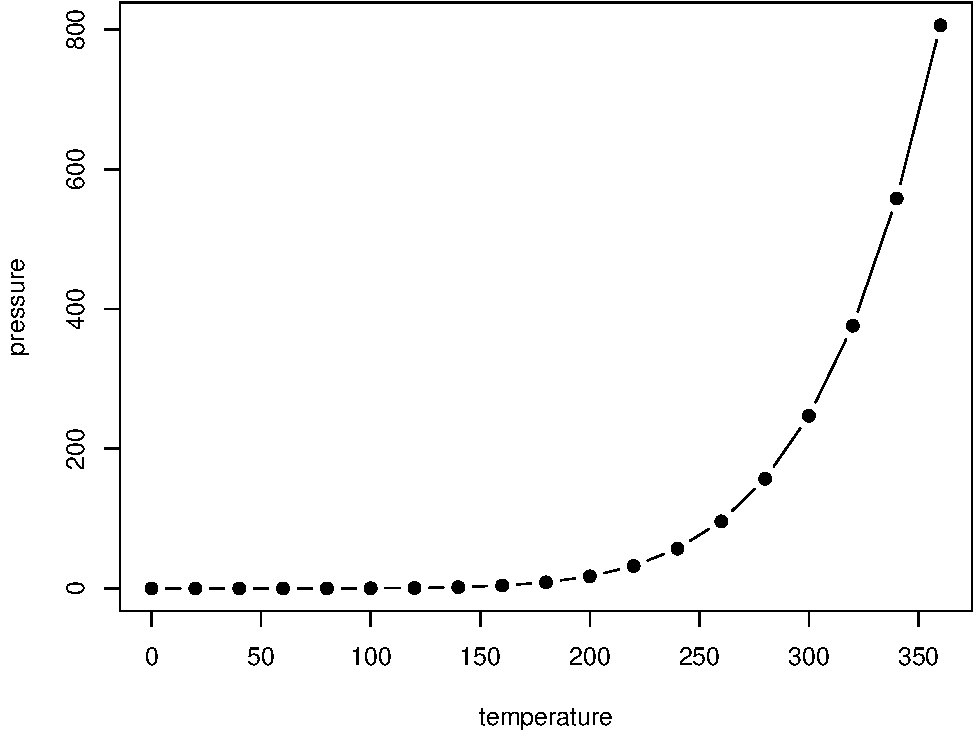
\includegraphics[width=0.8\linewidth]{_main_files/figure-latex/nice-fig-1} 

}

\caption{Here is a nice figure!}\label{fig:nice-fig}
\end{figure}

Don't miss Table \ref{tab:nice-tab}.

\begin{Shaded}
\begin{Highlighting}[]
\NormalTok{knitr}\SpecialCharTok{::}\FunctionTok{kable}\NormalTok{(}
  \FunctionTok{head}\NormalTok{(pressure, }\DecValTok{10}\NormalTok{), }\AttributeTok{caption =} \StringTok{\textquotesingle{}Here is a nice table!\textquotesingle{}}\NormalTok{,}
  \AttributeTok{booktabs =} \ConstantTok{TRUE}
\NormalTok{)}
\end{Highlighting}
\end{Shaded}

\begin{table}

\caption{\label{tab:nice-tab}Here is a nice table!}
\centering
\begin{tabular}[t]{rr}
\toprule
temperature & pressure\\
\midrule
0 & 0.0002\\
20 & 0.0012\\
40 & 0.0060\\
60 & 0.0300\\
80 & 0.0900\\
\addlinespace
100 & 0.2700\\
120 & 0.7500\\
140 & 1.8500\\
160 & 4.2000\\
180 & 8.8000\\
\bottomrule
\end{tabular}
\end{table}

\hypertarget{auxe7uxe3o-1---equipa-multidisciplinar}{%
\subsection{Ação 1 - Equipa Multidisciplinar}\label{auxe7uxe3o-1---equipa-multidisciplinar}}

\hypertarget{auxe7uxe3o-2-viva-as-fuxe9rias}{%
\subsection{Ação 2 -- Viva as Férias}\label{auxe7uxe3o-2-viva-as-fuxe9rias}}

\hypertarget{auxe7uxe3o-3-observatuxf3rio-monitorizauxe7uxe3o-e-apoio-ao-sucesso-escolar}{%
\subsection{Ação 3 -- Observatório monitorização e apoio ao sucesso escolar}\label{auxe7uxe3o-3-observatuxf3rio-monitorizauxe7uxe3o-e-apoio-ao-sucesso-escolar}}

\hypertarget{auxe7uxe3o-4-educauxe7uxe3o-5.0}{%
\subsection{Ação 4 -- Educação 5.0}\label{auxe7uxe3o-4-educauxe7uxe3o-5.0}}

\hypertarget{auxe7uxe3o-5-hora-de-programar}{%
\subsection{Ação 5 -- Hora de Programar}\label{auxe7uxe3o-5-hora-de-programar}}

\hypertarget{auxe7uxe3o-6-hora-de-experimentar}{%
\subsection{Ação 6 -- Hora de Experimentar}\label{auxe7uxe3o-6-hora-de-experimentar}}

\hypertarget{indicadores-de-resultado-e-realizauxe7uxe3o-da-operauxe7uxe3o-cofinanciada}{%
\section{Indicadores de resultado e realização da operação cofinanciada}\label{indicadores-de-resultado-e-realizauxe7uxe3o-da-operauxe7uxe3o-cofinanciada}}

\hypertarget{indicadores-especuxedficos-de-caracterizauxe7uxe3o-das-auxe7uxf5es}{%
\section{Indicadores específicos de caracterização das ações}\label{indicadores-especuxedficos-de-caracterizauxe7uxe3o-das-auxe7uxf5es}}

\hypertarget{impacto-da-pandemia-covid-19-na-execuuxe7uxe3o-das-atividades-e-projetos-programados}{%
\chapter{Impacto da pandemia Covid-19 na execução das atividades e projetos programados}\label{impacto-da-pandemia-covid-19-na-execuuxe7uxe3o-das-atividades-e-projetos-programados}}

You can add parts to organize one or more book chapters together. Parts can be inserted at the top of an .Rmd file, before the first-level chapter heading in that same file.

Add a numbered part: \texttt{\#\ (PART)\ Act\ one\ \{-\}} (followed by \texttt{\#\ A\ chapter})

Add an unnumbered part: \texttt{\#\ (PART\textbackslash{}*)\ Act\ one\ \{-\}} (followed by \texttt{\#\ A\ chapter})

Add an appendix as a special kind of un-numbered part: \texttt{\#\ (APPENDIX)\ Other\ stuff\ \{-\}} (followed by \texttt{\#\ A\ chapter}). Chapters in an appendix are prepended with letters instead of numbers.

\hypertarget{policy-recommendations}{%
\chapter{Policy recommendations}\label{policy-recommendations}}

\hypertarget{recomendauxe7uxf5es-sobre-o-combate-ao-insucesso-escolar}{%
\section{Recomendações sobre o combate ao insucesso escolar}\label{recomendauxe7uxf5es-sobre-o-combate-ao-insucesso-escolar}}

Footnotes are put inside the square brackets after a caret \texttt{\^{}{[}{]}}. Like this one \footnote{This is a footnote.}.

\hypertarget{recomendauxe7uxf5es-metodoluxf3gicas-para-os-programas-de-combate-ao-insucesso-escolar-cofinanciados-no-quadro-2021-2027}{%
\section{Recomendações (metodológicas) para os programas de combate ao insucesso escolar cofinanciados no quadro 2021-2027}\label{recomendauxe7uxf5es-metodoluxf3gicas-para-os-programas-de-combate-ao-insucesso-escolar-cofinanciados-no-quadro-2021-2027}}

Reference items in your bibliography file(s) using \texttt{@key}.

For example, we are using the \textbf{bookdown} package \citep{R-bookdown} (check out the last code chunk in index.Rmd to see how this citation key was added) in this sample book, which was built on top of R Markdown and \textbf{knitr} \citep{xie2015} (this citation was added manually in an external file book.bib).
Note that the \texttt{.bib} files need to be listed in the index.Rmd with the YAML \texttt{bibliography} key.

The RStudio Visual Markdown Editor can also make it easier to insert citations: \url{https://rstudio.github.io/visual-markdown-editing/\#/citations}

\hypertarget{recomendauxe7uxf5es-sobre-a-atuauxe7uxe3o-das-comunidades-intermunicipais}{%
\section{Recomendações sobre a atuação das Comunidades Intermunicipais}\label{recomendauxe7uxf5es-sobre-a-atuauxe7uxe3o-das-comunidades-intermunicipais}}

\hypertarget{referuxeancias-bibliogruxe1ficas-e-eletruxf3nicas}{%
\chapter*{REFERÊNCIAS BIBLIOGRÁFICAS E ELETRÓNICAS}\label{referuxeancias-bibliogruxe1ficas-e-eletruxf3nicas}}
\addcontentsline{toc}{chapter}{REFERÊNCIAS BIBLIOGRÁFICAS E ELETRÓNICAS}

\hypertarget{equations}{%
\section{Equations}\label{equations}}

Here is an equation.

\begin{equation} 
  f\left(k\right) = \binom{n}{k} p^k\left(1-p\right)^{n-k}
  \label{eq:binom}
\end{equation}

You may refer to using \texttt{\textbackslash{}@ref(eq:binom)}, like see Equation \eqref{eq:binom}.

\hypertarget{theorems-and-proofs}{%
\section{Theorems and proofs}\label{theorems-and-proofs}}

Labeled theorems can be referenced in text using \texttt{\textbackslash{}@ref(thm:tri)}, for example, check out this smart theorem \ref{thm:tri}.

\begin{theorem}
\protect\hypertarget{thm:tri}{}\label{thm:tri}For a right triangle, if \(c\) denotes the \emph{length} of the hypotenuse
and \(a\) and \(b\) denote the lengths of the \textbf{other} two sides, we have
\[a^2 + b^2 = c^2\]
\end{theorem}

Read more here \url{https://bookdown.org/yihui/bookdown/markdown-extensions-by-bookdown.html}.

\hypertarget{callout-blocks}{%
\section{Callout blocks}\label{callout-blocks}}

The R Markdown Cookbook provides more help on how to use custom blocks to design your own callouts: \url{https://bookdown.org/yihui/rmarkdown-cookbook/custom-blocks.html}

  \bibliography{book.bib,packages.bib}

\end{document}
